\chapter{8. Conclusions and Future Work}

\begin{quote}
\textit{The World Health Organization considers air quality to be the single leading environmental cause of death around the world.  One in eight deaths worldwide are linked to poor air quality.} \newline
\end{quote}


\section{Applications}
-example and provocation to citizen sensing community.
-datastore for big data sharing.  
-extensible for any type of algorithm, particularly designed for learning algorithms to intelligently calibrate and predict accuracy.
-EPA data sharing.  Data sharing in general.
-EPA testing of cheap sensors.
-towards personal tracking, intelligent systems.  highly scalable.
-sell as platform/stamp of approval, change/define a new validation process for new sensors.  all new consumer sensors push data to chain and are independently verified.  Verified for regions of the country, verified for conditions, verified with a ranking of accuracy not just a yes or no.


\section{Insights}

-insight into shuffled vs. folded data, whether you've tested long enough in one climate.
-insights into how these things break down
-insights into feature reduction - explore how to build a cheap system, look at how strong a relationship is, and if it breaks in a statistically reliable way, inform our decisions moving forward.  Is it corroborated across multiple feature reduction methods?
-insight into feature reduction - explore the underlying mechanisms that might break a system down 
-insight into speed of sensor reaction, and what that means for building a system like this, how it interacts with health.
-insight into cheap sensors, contrast SQMD with my results.
-insight into windspeed.
-insight into data sharing and backend design.
-usefulness of accuracy of predictions?  not large now.  Would have to be statistical techniques.
-insight into overall system feasibility.


\section{Future Work}

as with any good project, this thesis begets as many questions as it answers.
-wind sensing.
-pollen, scrape. no api.  realtime Traffic data a la google maps.  Traffic type data based on road type (estimate of heavy deasel etc).  Construction.  Map and distance from a street, buildings, etc.  Age of infrastructure.  SES of neighborhood as a predictor of car age and emissions.  Aeris.
-mount on Aclima car.
-more intelligent input data - distance to road, vibration, speed traveling, traffic pattern data.
-approached by a few people will to test.
-more data, test with newer sensors.
-try other machine learning techniques, time-dependent, deep-learning.  all possible.
-data backend infrastructure buildout, promote in community.
-more tools for backend crawling.
-help educate communities.
-help automate testing for big organizations.
-build out recommedation system for devices that perform well in different environments.
-build out trustworthiness system for devices based on make/model to characterize interpart variability.
-statistical tools for combining sensor data - spikes missing?  is there a way to predict frequency/intensity in an area by looking at closest high quality sensor?


\section{Summary}

-hand waving goal - a sensor that learns when it's around a better sensor what conditions it can be trusted.  As you carry it away from that sensor, it predicts what measurements it makes are trustworthy, and what measurements are not.

we set out to achieve x.  we did.  This shows promise, this was lacking.  many future directions.

Did (1). Did (2).  Did (3).  Steps toward an interesting system.

Right now this is immediately useful for automatic calibration, and for showing systemic errors and correlates.  There needs to be a human in the loop that looks and understands the physics right now, but with enough training and another layer of abstraction it may be possible for the machine to identify common issues (common cross-sensitivities, optical issues around fog or road dust, typical deficiencies for certain types of sensors to temperature/humidity/response time).



%here's text referencing the (Table \ref{tab:sample_table}).
%
%\begin{table}
%  \centering
%  \begin{tabular}{l l l l l}
%    Column A & Column B & Column C & Column D & Column E \\
%    \toprule
%    A & B & C & D & E
%  \end{tabular}
%  \caption{A meaningless table}
%  \label{tab:sample_table}
%\end{table}

%Here's text referencing the margin figure (Figure \ref{fig:spin_margin}).
%
%\marginnote{\textbf{Margin Note:} Check it out, here's a margin note.}
%
%\begin{marginfigure}[{-10cm}]
% 	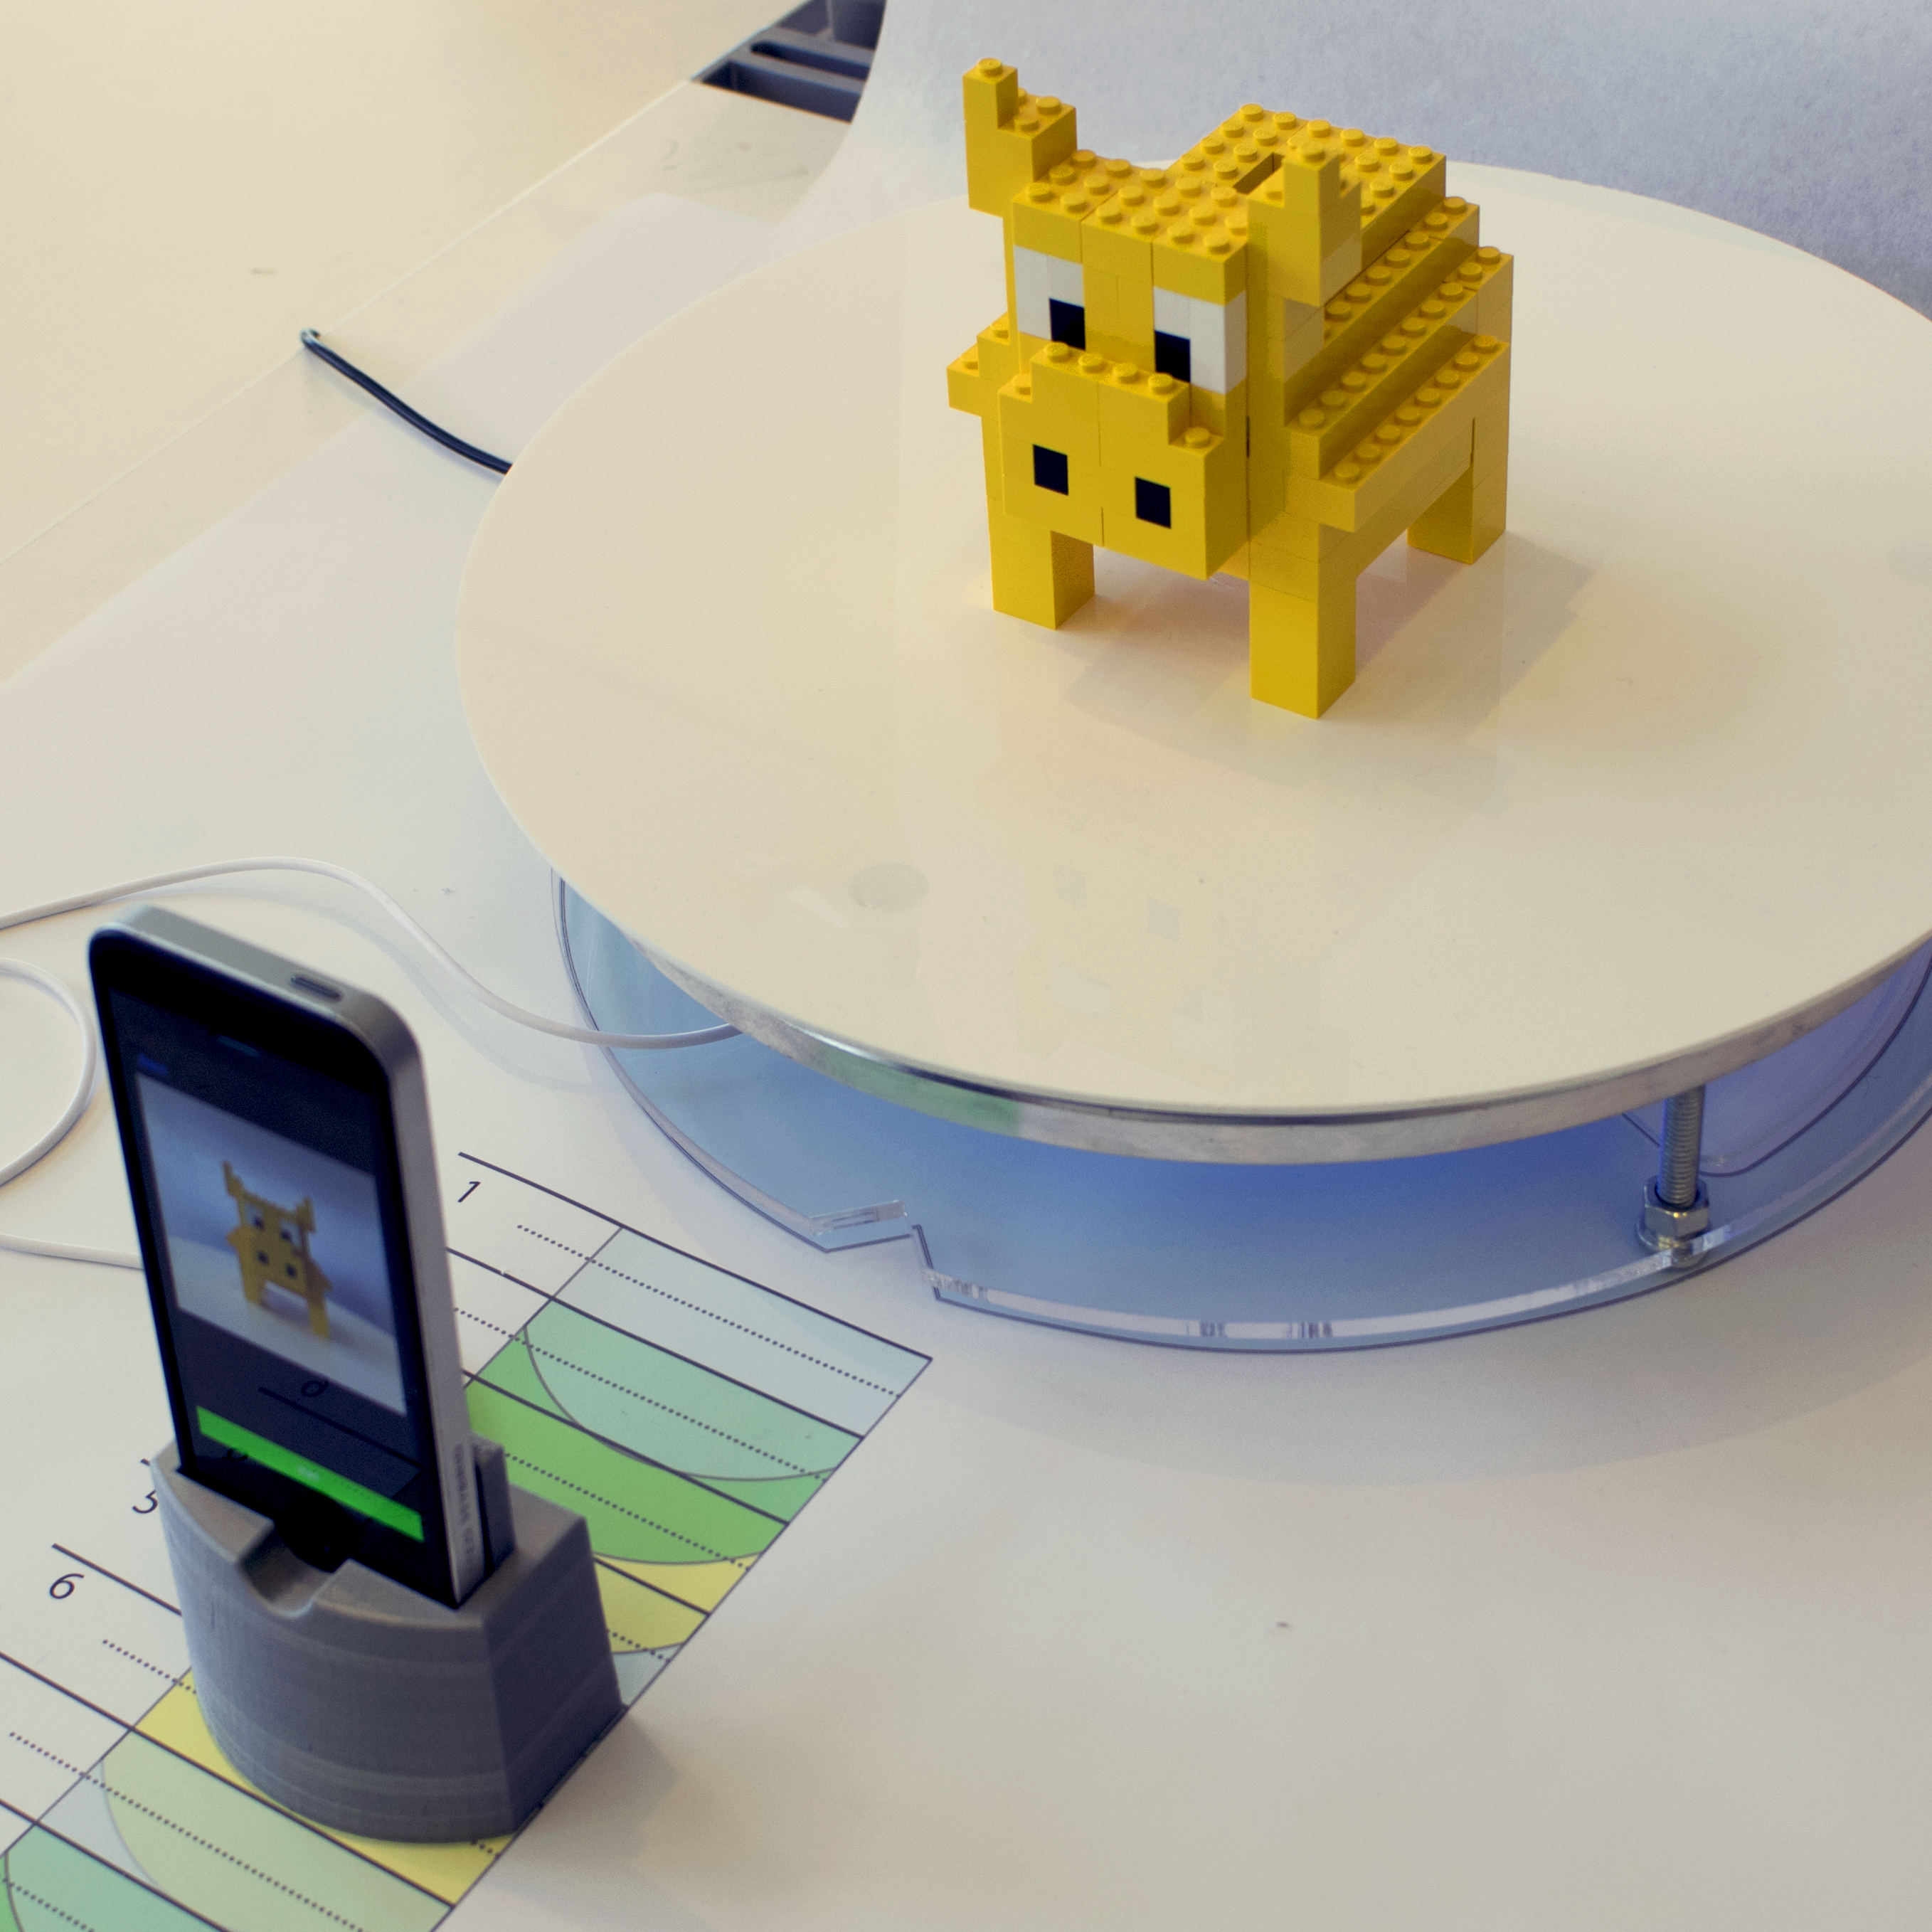
\includegraphics[width=\textwidth]{chap1/spin}               
% 	 \caption{Check it out, it's a Spin margin figure \url{spin.media.mit.edu}}
%  	\label{fig:spin_margin}
%\end{marginfigure}

%\begin{figure}[htb]
% 	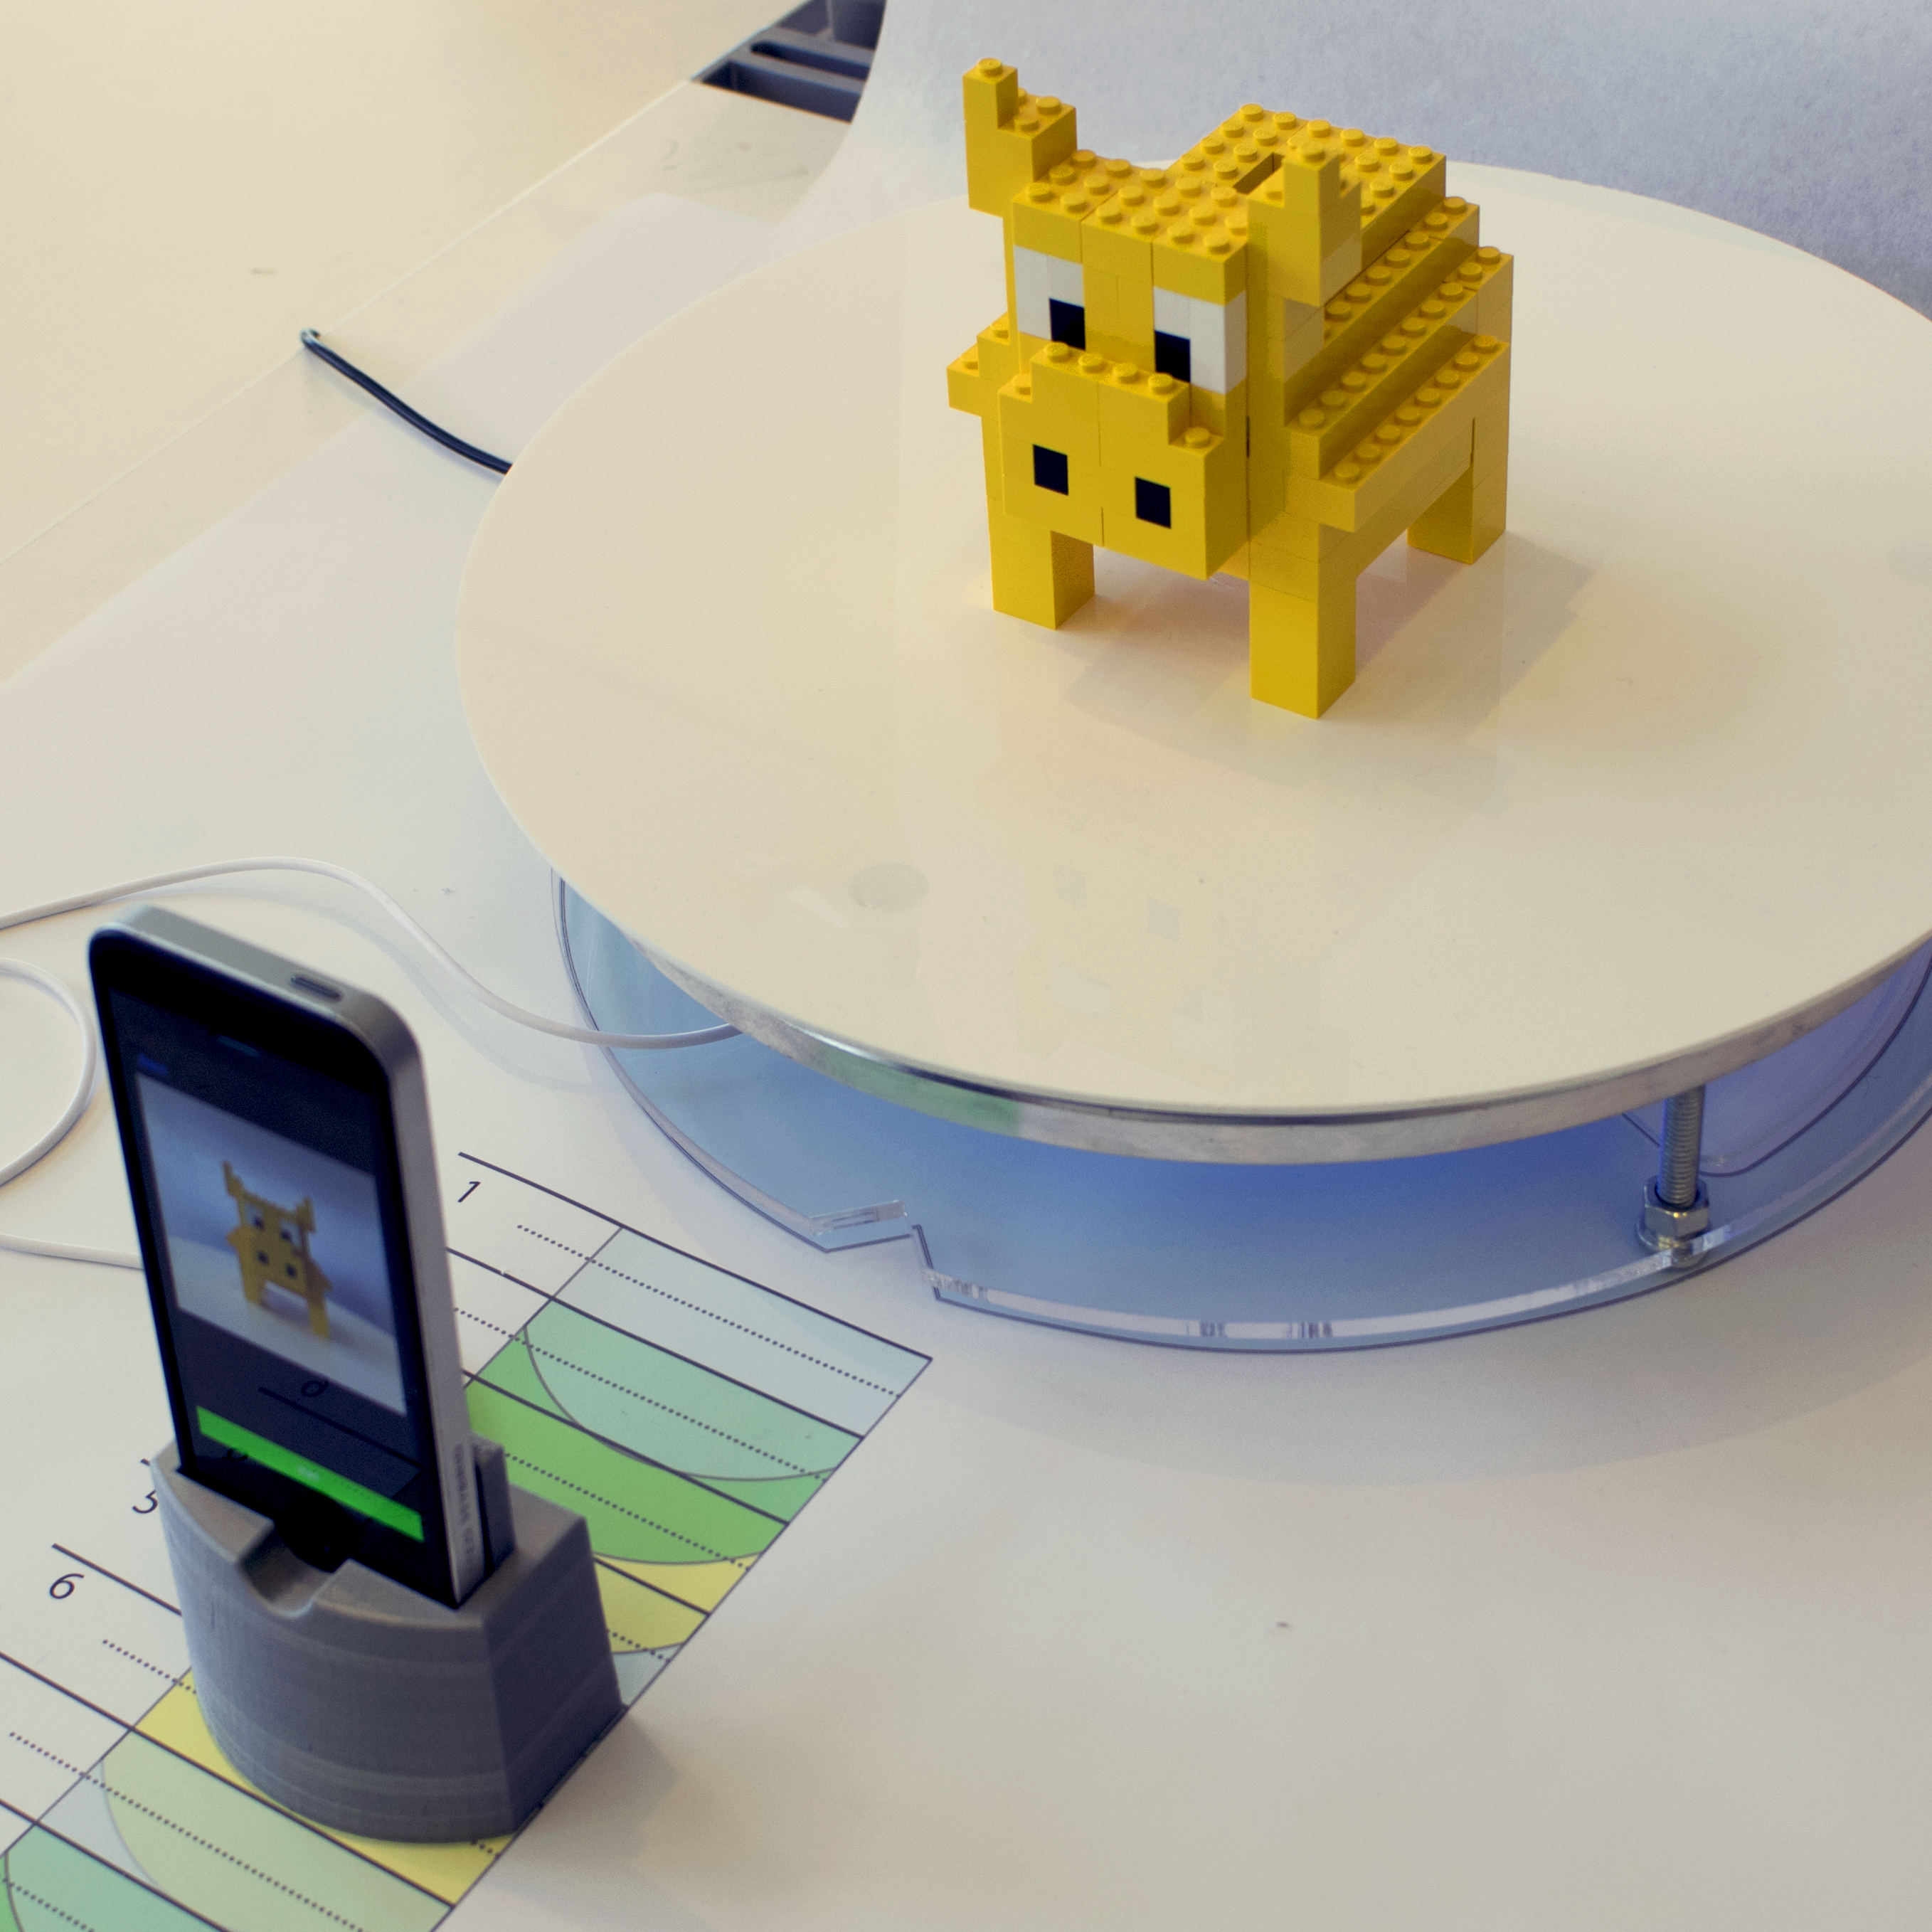
\includegraphics[width=\textwidth]{chap1/spin}               
% 	 \caption{Check it out, it's a Spin \url{spin.media.mit.edu}}
%  	\label{fig:spin}
%\end{figure}
